% Ajit and Craig's section

\graphicspath{{11-Absorber/Figures/}}

\section{Liquid-Hydrogen Absorber}
\label{Sect:Absorber}

\subsection{Introduction}

The absorber vessel consist of a cylindrical aluminium body sealed with
two thin aluminium end windows, as shown in figure~\ref{Fig:AbsorberVessel:Diag}.
\begin{figure}[htb!]
  \begin{center}
    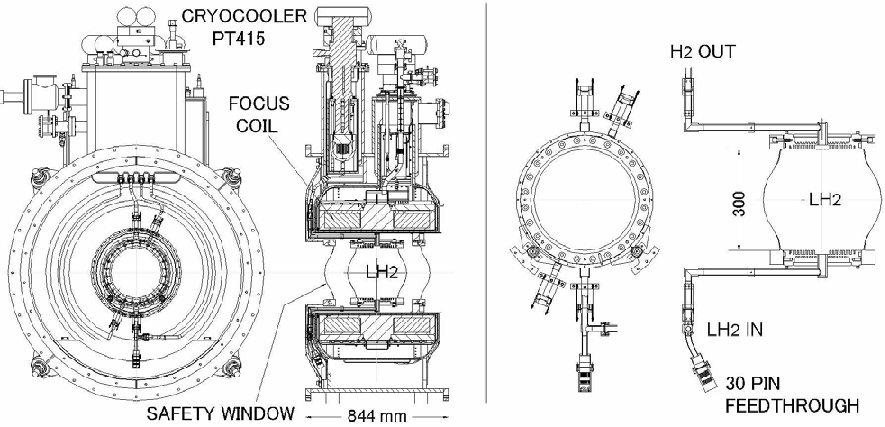
\includegraphics[width=0.75\textwidth]{11-Absorber/Figures/AFC-drwng.pdf}
  \end{center}
  \caption{
    Left panel: Drawing of the absorber/focus-coil (AFC) module showing the principal components. Right panel: detail of the liquid-hydrogen absorber vessel.
  }
  \label{Fig:AbsorberVessel:Diag}
\end{figure}
The absorber vessel has a volume of 22\,l of liquid with body dimensions with
an inner diameter of 300\,mm and a length between its end
flanges of 230\,mm.  
The length along the central axis between the two domes of the thin aluminium end
windows was 350\,mm~\cite{1748-0221-13-09-T09008}.

%%%%%%%%%%%%%%%%%%%%%%%%%%%%%%%%%%%%%%%%%%%%%%%%%%%%%%%%%%%%%

\subsection{Systematic studies}

\subsubsection{Variation of the density of liquid-hydrogen due to varying temperature and pressure}
\label{SubSect:Absorber_temperature}

The energy lost by a muon travelling through the liquid-hydrogen absorber depends on the path length the
muon travelled through and on the density of the liquid-hydrogen. The density of liquid-hydrogen is a function of temperature and pressure. 
The temperature of the vessel was recorded by eight LakeShore Cernox 1050 SD sensors with a resolution of 0.1\,K.
Four of the sensors were used solely as temperature sensors, while the other four were used also as level
sensors to ensure the liquid-hydrogen reached the top of the vessel.
They were arranged in pairs
%(Fig.\ref{Fig:AbsorberVessel:BdyPhoto})
with two mechanically clamped at the  top of the vessel, two at a rotation of ${45}^{\circ}$, a further two at a further rotation of
${90}^{\circ}$ and a final two at a further rotation of ${45}^{\circ}$ to be at the bottom of the vessel.

Cooldown and liquefaction were completed slowly over eight days at a pressure of 1.15\,Bar after which the vessel's pressure was lowered to 1.085\,Bar~\cite{1748-0221-13-09-T09008}. The vessel then remained in this steady-state equilibrium until the venting process began. During this process the cryocooler was switched off and the heaters were switched on, delivering a nominal power of 50\,Watt to the absorber vessel. This resulted in an increase in pressure and temperature until the temperature stabilised at the boiling point. A rapid increase in temperature was observed once all the liquid-hydrogen had boiled off.

The sensors have a typical accuracy of $\mathrm{\pm}$\,9\,mK and a long-term stability of $\mathrm{\pm}$\,12\,mK at 20\,K. The magnetic-field dependent temperature error at 2.5\,T is 0.04\%, $\Delta$T/T, equivalent to $\mathrm{\pm}$\,8\,mK at 20\,K~\cite{CernoxRTDs}\cite{TemperatureMeasurement}. These are the quoted uncertainties given by the manufacturer of the sensors. The importance of magnetic fields on temperature measurements is that they cause reversible calibration shifts: when the magnetic field is removed, the sensors return to their original calibration.

To reduce the uncertainty in the liquid-hydrogen density a calibration procedure was devised using the boiling point: the corrected temperature reading was found by applying a cut-off correction, a magnetic field correction based on the focus coil current and mode, a correction for the non-linearity of the sensors, and a boiling point scaling factor~\cite{NOTE524}. 
%\begin{table}
%\scriptsize
%  \caption{
%    Temperature coefficient scaling factor for each sensor calculated by dividing the temperature reading (adjusted for cut-off coefficient and magnetic field) by the vaporisation temperature at that pressure
%  }
%  \label{tab:temperature}
%  \begin{center}
%    \begin{tabular}{|c c c c c c c c c|}
%    \hline
%
%Mode      & LSA & LSB & LSD & LSE & TSA & TSB & TSD & TSE     \rule{0pt}{10pt} \\
%\hline
%T/T${}_\textrm{Boiling}$ &  1.010581837 & 0.989245608 & 1.003371485 & 1.008424313 & 1.027755673 & 1.003697746 & 0.9784283 & 1.015526132\\
%
%    \hline
%    \end{tabular}
%  \end{center}
%\end{table} 

\begin{figure}[htb!]
  \begin{center}
  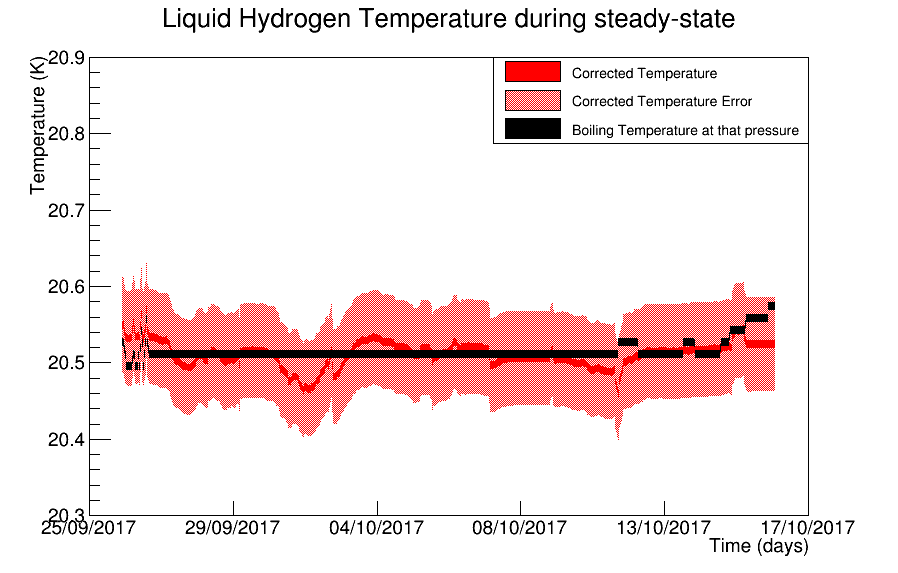
\includegraphics[width=0.80\textwidth]{11-Absorber/Figures/SteadyState60mK.png}
  \end{center}
  \caption{Average LH2 temperature recorded by the sensors during the steady-state period. After applying all the correction factors the temperature remains at or close to the boiling point temperature.}
  \label{Fig:TempCalibrated}
\end{figure}
 
The boiling point of hydrogen at 1.085\,Bar is 20.511\,K. There are however a number of uncertainties.
The sensors have a total uncertainty of 17\,mK (9\,mK accuracy, 12\,mK stability, 8\,mK magnetic). The non-linearity of the sensors adds 0.03\,K.
The temperature scaling and magnet current correction factors also have an associated error as they are based on the 0.1K resolution.
For example, a calibrated sensor at boiling temperature and 1.505\,Bar should read 21.692\,K, but can only read 21.65\,K (21.6\,K cut-off plus 0.05 cut-off correction) i.e. it is off by 0.042\,K. The pressure sensors have an uncertainty of $\mathrm{\pm}$\,5\,mBar which equates to $\mathrm{\pm}$\,0.016\,K during steady state.
The pressure uncertainty ($\mathrm{\pm}$\,5\,mBar) adds another uncertainty to the temperature calibration constants of $\mathrm{\pm}$\,0.014\,K. Collectively, all these uncertainties add up to 0.2\,K for each sensor.
 
For our steady state condition the liquid-hydrogen was close to the boiling temperature of liquid parahydrogen~\cite{NOTE524}. The average temperature of the eight sensors during steady-state was (20.51\,$\mathrm{\pm}$\,0.07)\,K at 1.085\,Bar (figure~\ref{Fig:TempCalibrated}) and allows us to determine the uncertainty in the density as (70.53\,$\mathrm{\pm}$\,0.08)\,kg/m$^{3}$.
 

\subsubsection{Contraction of the absorber vessel due to cooling}
\label{SubSect:Absorber_Contraction}

The aluminium absorber vessel was cooled from room temperature to the operating temperature of the
experiment (20.51\,K), which resulted in the vessel contracting. The linear contraction of
Al-6061 as it is cooled from 293K is given by:

\begin{equation}
  \alpha =-4.1277\times {10}^{-3}\mathrm{T}-3.0389\times {10}^{-6}\mathrm{T}^2+8.7696\times {10}^{-8}\mathrm{T}^3-9.9821\times {10}^{-11}\mathrm{T}^4
\end{equation}
where T is the operating temperature~\cite{Hardin}. The equation is a line of best fit of data collated by NIST
(National Institute of Standards and Technology) and has an associated curve fit error of 4\%.
At the MICE operating temperature, this corresponds to a linear contraction of the vessel along each plane of 0.415\%,
resulting in a warm bore length (350\,mm) contraction of (1.45\,$\mathrm{\pm}$\,0.05)\,mm. The vessel was held suspended in place, meaning the vessel was free to contract along each plane without restriction, since the vessel was free to contract within the warm bore of the focus coil.

\subsubsection{Deflection of absorber vessel windows due to internal pressure}
\label{SubSect:Absorber_pressure}

To minimise energy loss and Coulomb scattering by the absorber vessel, the windows were kept as thin as
possible. They must however not rupture when handling any internal pressure they are subjected to. For
safety considerations~\cite{1748-0221-13-09-T09008}\cite{Ishimoto} it was necessary for the liquid-hydrogen
circuit to be pressurised above atmospheric pressure to prevent air ingress. The vessel must also be
capable of handling up to 1.5 Bar, the relief valve set pressure.

These pressures resulted in a deflection of the absorber windows and were modelled using
ANSYS~\cite{NOTE155}. The uncertainty in the model's window deflection was 20\%. It showed a linear
expansion of the window deflection with pressure up to 2 Bar when the windows begin to yield.
The pressure sensors were accurate to $\mathrm{\pm}$\,5\,mBar (0.25\% of 2\,Bar). At (1085\,$\mathrm{\pm}$\,5)\,mBar, the typical MICE operating pressure, this corresponded to a deflection of (0.5374\,$\mathrm{\pm}$\,0.1076)\,mm (model uncertainty) $\mathrm{\pm}$\,0.0022\,mm (sensor uncertainty) at the centre of
the absorber window.


\subsubsection{Variation of the absorber vessel window thicknesses}
\label{SubSect:Absorber_thickness}

The amount of energy loss and cooling experienced by a muon passing through the absorber depends on the amount of
aluminium and liquid-hydrogen traversed. There were four windows, two absorber wall windows of the vessel and two safety windows.
%(Windows 002, 003, 009 and 012 from table \ref{tab:summary}) 

At the centre of the absorber, the total amount of aluminium the muon beam passes through was (785\,$\mathrm{\pm}$\,13)\,$\mu$m, a variance of 1.68\%. However, as the windows were thin, the effects on energy loss were negligible. A 200\,MeV/$c$ muon passing along the central axis of an empty absorber loses 0.345\,MeV, which introduces a 0.006\,MeV uncertainty on energy loss.


\subsubsection{Total Systematic Uncertainty on Energy Loss}
\label{SubSect:Absorber_total}

In total there are three main contributions to the systematic uncertainty of the liquid-hydrogen absorber on energy loss. The contraction of the absorber and deflection of the absorber window due to internal pressure reduces the central warm bore length by (0.4\,$\mathrm{\pm}$\,0.2)\,mm.
%(Eq.~\ref{Totaldeflection}) 
%\begin{equation}
%    1.4525\ \left(\pm \ 0.0581\right)-2\left(0.5374\left(\pm 0.1098\right)\right)=0.3777\pm 0.1629=0.4mm\pm 0.2mm
%\label{Totaldeflection}    
%\end{equation}

The combined absorber window's thickness variation at the centre of the absorber is 13\,$\mu$m. The average temperature during the steady state period of the experiment when the pressure remained constant at (1085\,$\mathrm{\pm}$\,5)\,mBar is (20.51\,$\mathrm{\pm}$\,0.07)\,K corresponding to a liquid-hydrogen density of (70.53\,$\mathrm{\pm}$\,0.08)\,kg/m$^{3}$.

The energy loss is momentum dependent, as each particle will lose a different amount of energy passing through the absorber. Tables \ref{tab:Aluminium} and \ref{tab:Hydrogen} show the energy loss at various momenta for aluminium and for various densities of liquid-hydrogen, respectively~\cite{AtomicAluminium}\cite{AtomicHydrogen}\cite{MuonAluminium}\cite{MuonliquidHydrogen}.
277\,MeV/$c$ and 344\,MeV/$c$ are the minimum ionization momenta of aluminium and liquid-hydrogen, respectively.


\begin{table}[htb!]
  \caption{
    Energy Loss for aluminium (Al-6061) at various nominal muon momenta with a density of 2.699\,g/cm$^{3}$.
  }
  \label{tab:Aluminium}
  \begin{center}
    \begin{tabular}{|c c c c c|}
    \hline

Momentum (MeV/$c$) & 100 & 140 & 200 & 277     \rule{0pt}{14pt} \\
\hline
{Mass Stopping Power (MeVg${}^{-1}$cm${}^{2}$)} & 1.798 & 1.688 & 1.630 & 1.615
\\
{Stopping Power (MeVcm${}^{-1}$)} & 4.8528 & 4.556 & 4.3994 & 4.3589
\\

    \hline
    \end{tabular}
  \end{center}
\end{table} 

\begin{table}
  \caption{
    Energy loss for liquid-hydrogen at various densities (0.0703 to 0.0708 g/cm${}^{3}$) and various muons momenta.}
  \label{tab:Hydrogen}
  \begin{center}
    \begin{tabular}{|c c c c c|}
    \hline

Momentum & 100 & 140 & 200 & 344     \rule{0pt}{14pt} \\
\hline
{Mass Stopping Power} & 4.568 & 4.267 & 4.104 & 4.034 \\
{Stopping Power }(at $\rho$=0.0703)\textbf{} & 0.3211 & 0.29997 & 0.2885 & 0.28359\\
{Stopping Power }(at $\rho$=0.07054)\textbf{} & 0.3222 & 0.30099 & 0.2895 & 0.2846 \\
{Stopping Power }(at $\rho$=0.07078)\textbf{} & 0.3233 & 0.3020 & 0.29048 & 0.2855 \\
{Stopping Power }(at $\rho$=0.0708)\textbf{} & 0.3234 & 0.3021 & 0.29056 & 0.2856 \\
    \hline
    \end{tabular}
  \end{center}
\end{table} 


During MICE, muon beam of momentum 140, 170, 200 and 240\,MeV/$c$ were used. The energy loss and its uncertainty were calculated. The calculation used a central bore length of (349.6\,$\mathrm{\pm}$\,0.2)\,mm, a total window thickness of (0.785\,$\mathrm{\pm}$\,0.013)\,mm and a liquid-hydrogen density of (70.53\,$\mathrm{\pm}$\,0.08)\,kg/m$^{3}$ for a particle travelling straight through the centre of the absorber.

For a 140\,MeV/$c$ muon particle this corresponds to an energy loss of (10.88\,$\mathrm{\pm}$\,0.02)\,MeV, while for a 200\,MeV/$c$ muon particle this corresponds to an energy loss of (10.44\,$\mathrm{\pm}$\,0.02)\,MeV. In terms of energy loss, the systematic error is 0.2\%. This is for a particle travelling along the central axis of the absorber. A muon travelling through the absorber in the presence of a magnetic field would take a different path and thus would traverse a different length of aluminium and liquid-hydrogen.
 
%%%%%%%%%%%%%%%%%%%%%%%%%%%%%%%%%%%%%%%%%%%%%%%%%%%%%%%%%%%%%%%%%%%55 
% Scott's section 
%\subsection{Systematic effect on the Scattering Analysis}
%\label{SubSect:Absorber_E}

%\subsection{Validation of the absorber model in MAUS}
%\label{SubSect:Absorber_Validation}

%As a test of the absorber model, an analysis has been performed to measure the muon energy loss in the LiH and liquid-hydrogen absorbers and compare it to the energy loss predicted by the MC.  A previous analysis measured this effect using only the TOF detectors~\cite{rhys_thesis} and found good agreement in the mean energy loss, but did not have the precision to measure the shape of the distribution.  In this updated energy loss analysis, the addition of the trackers allows better PID, slightly improved momentum measurements upstream compared to the TOF0-TOF1 measurement, and significantly improved momentum measurements downstream compared to the TOF1-TOF2 estimate.

%Muons are selected using the particle ID described in Section~\ref{Sect:PID}.  The muons' upstream momentum (before the absorber) is measured using an average of the momentum measured by the tracker (at the plane nearest to the absorber) and the momentum calculated using the TOF0 to TOF1 flight time.  This average is weighted by the expected resolution of the two measurements. (The resolutions are roughly the same for low-momentum muons, but the TOF measurement of momentum is less accurate for higher-momentum muons.)  The muons' downstream momentum is measured solely using the dowstream tracker.

%The momentum change is measured for each beam momentum both with and without an absorber present.  The LiH `empty' measurement is done with no absorber present, while the liquid-hydrogen `empty' measurement is done with the hydrogen vessel in place, but not filled.  The measurement with no absorber is used to find the resolution of the detector, and the measurement with a full absorber should then be a convolution of the true loss in the absorber and this resolution.

%In order to extract the true momentum loss in the absorber, the `empty absorber' result is modeled by a gaussian distribution.  The `full absorber' measurement is then fit to a convolution of a the true momentum loss (a landau distribution with free parameters) and the resolution of the detector (a gaussian distibution with parameters fixed by the `empty absorber' fit).

%\begin{figure}
%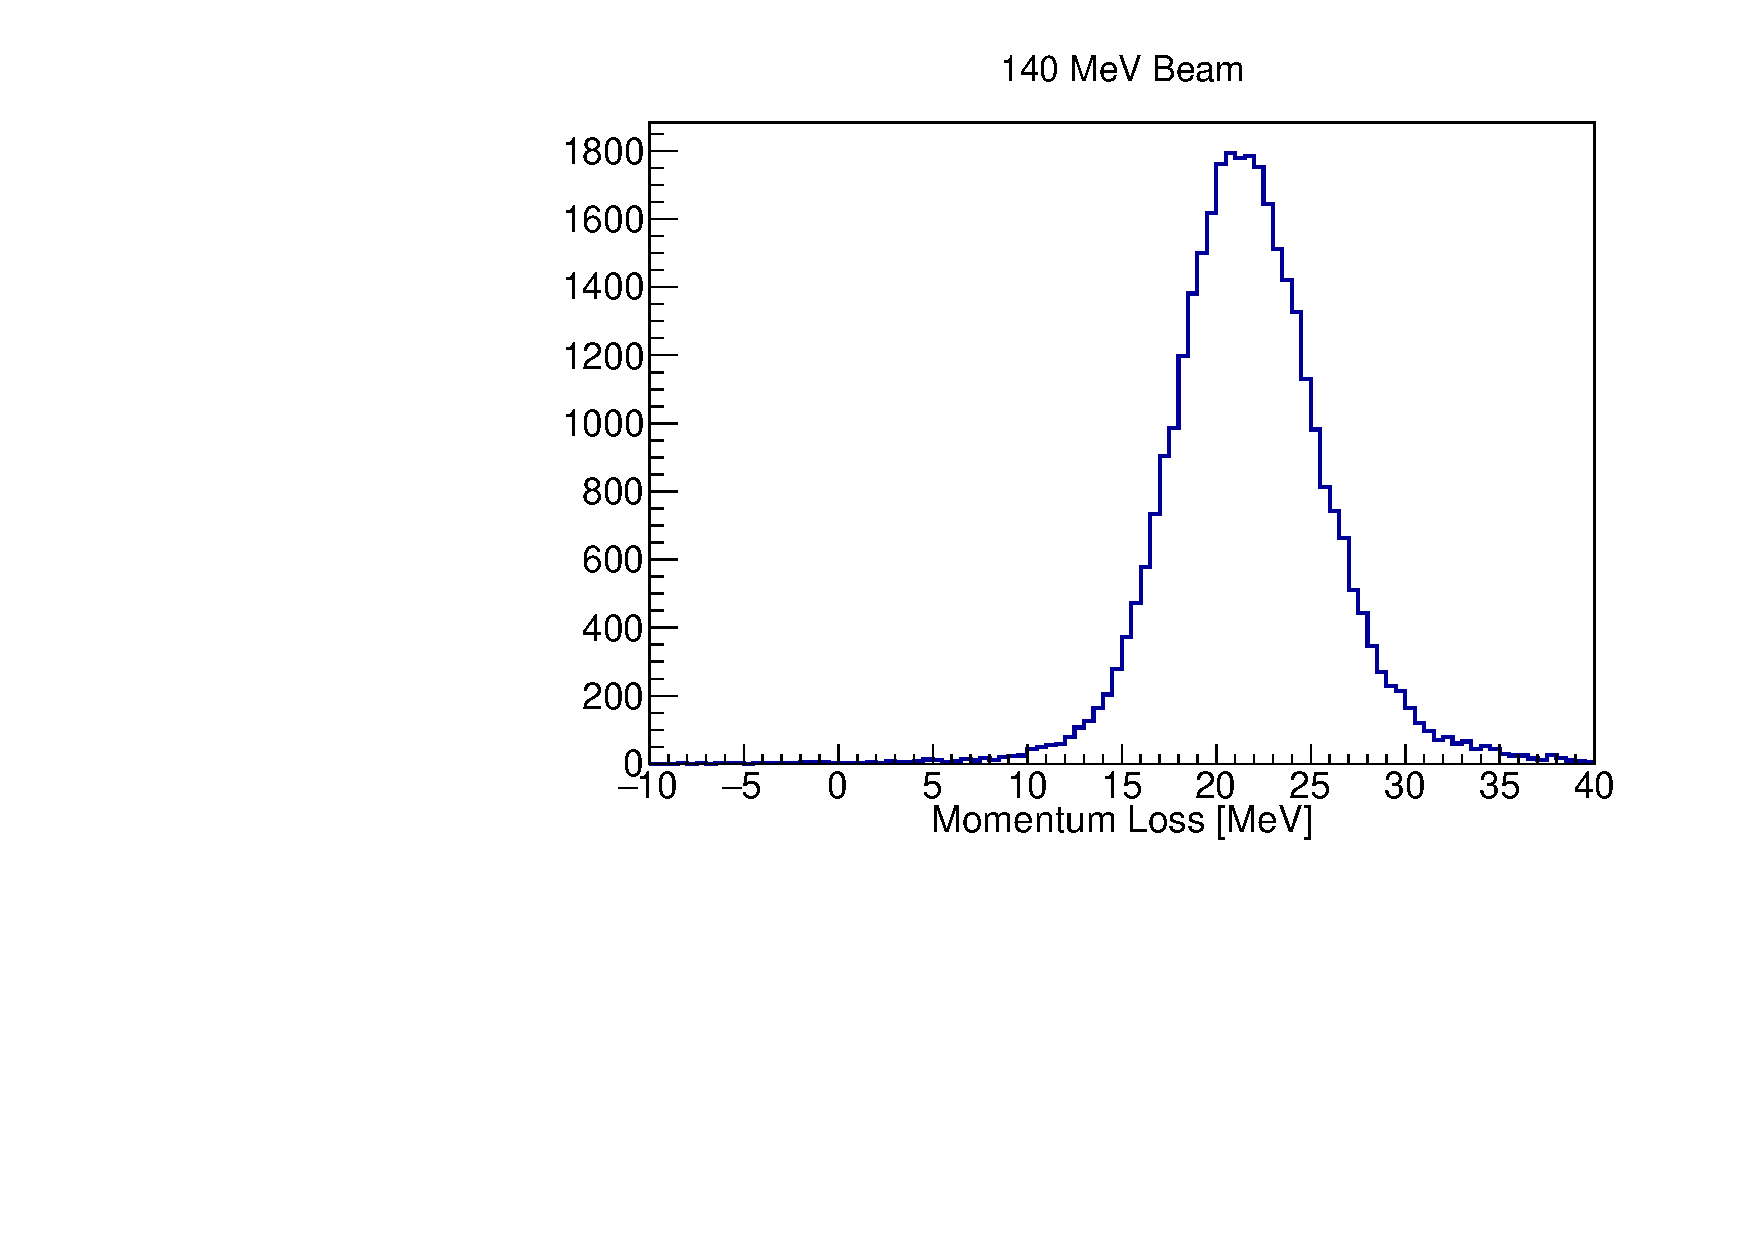
\includegraphics[width=0.45\textwidth]{11-Absorber/Figures/raw_140.pdf}\hfil
%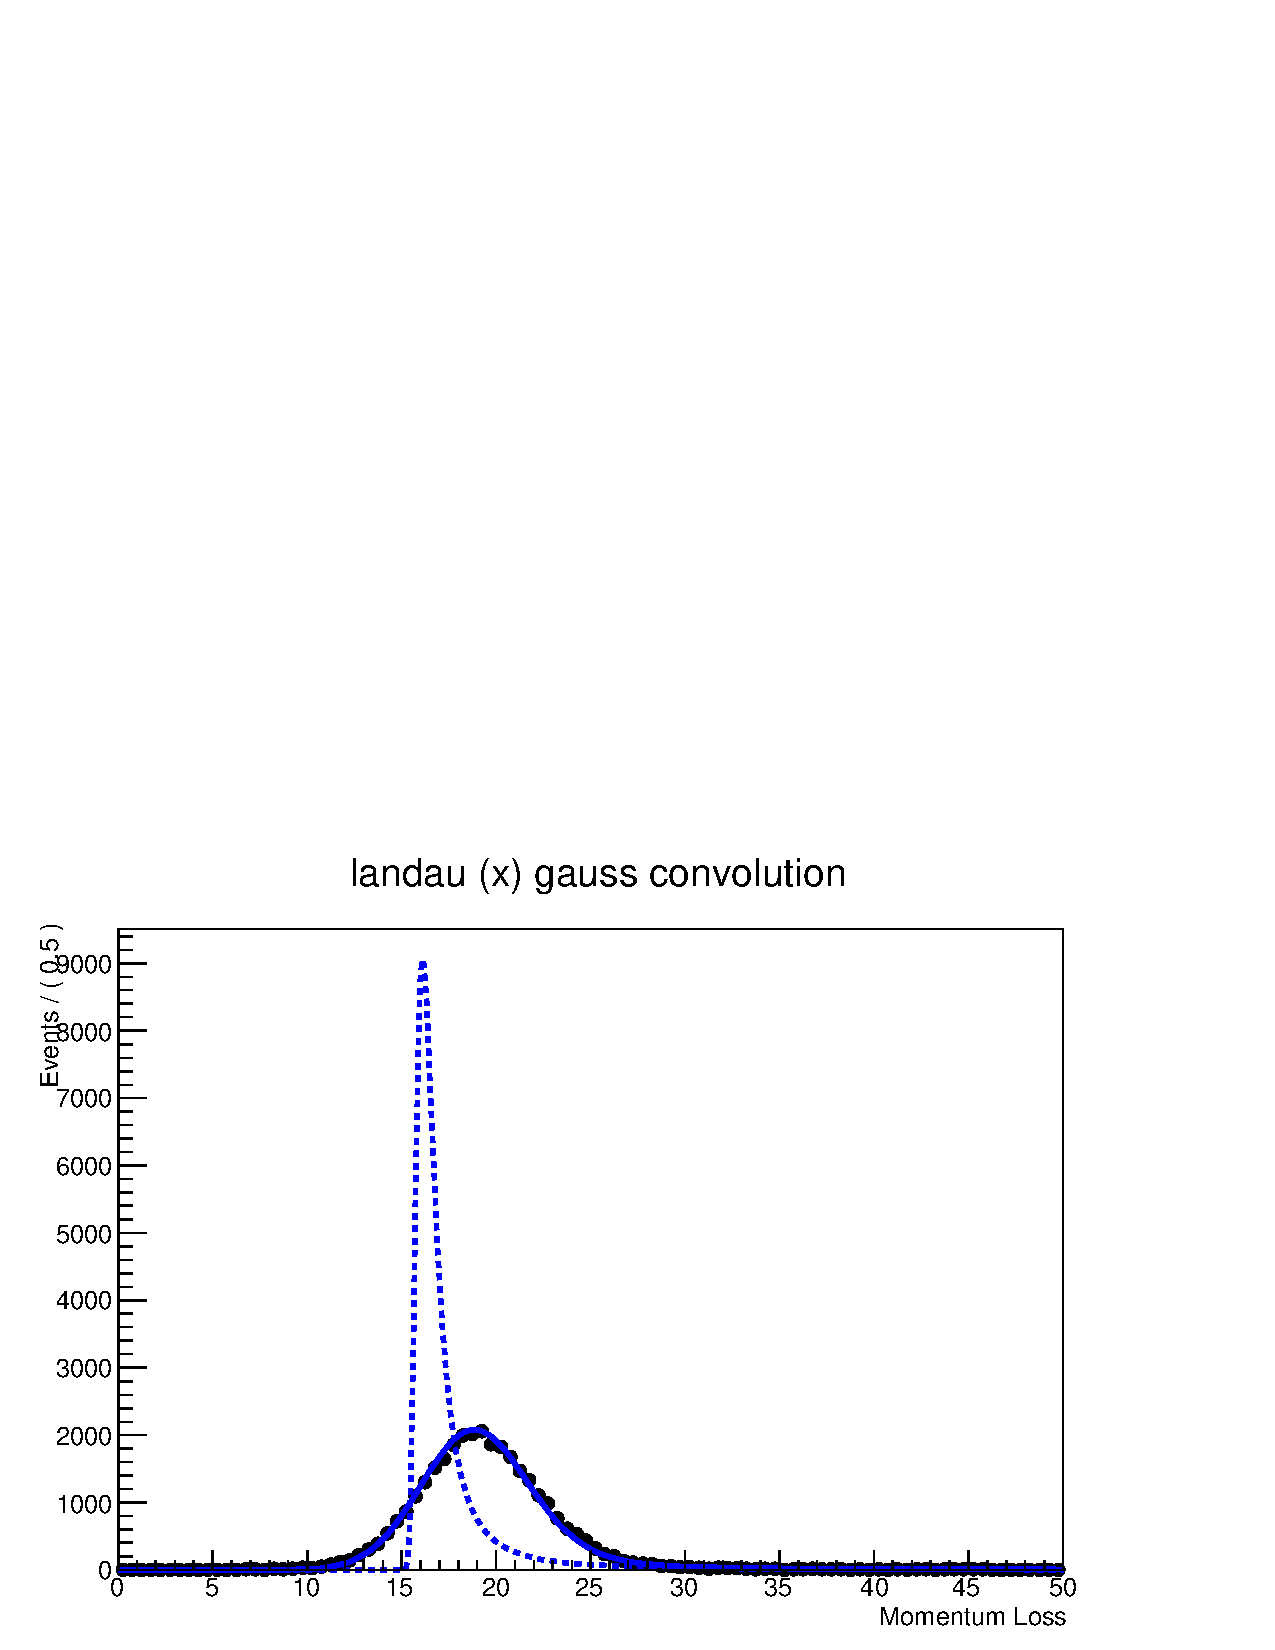
\includegraphics[width=0.45\textwidth]{11-Absorber/Figures/deconv_140.pdf}
%\vspace{-5cm}
%
%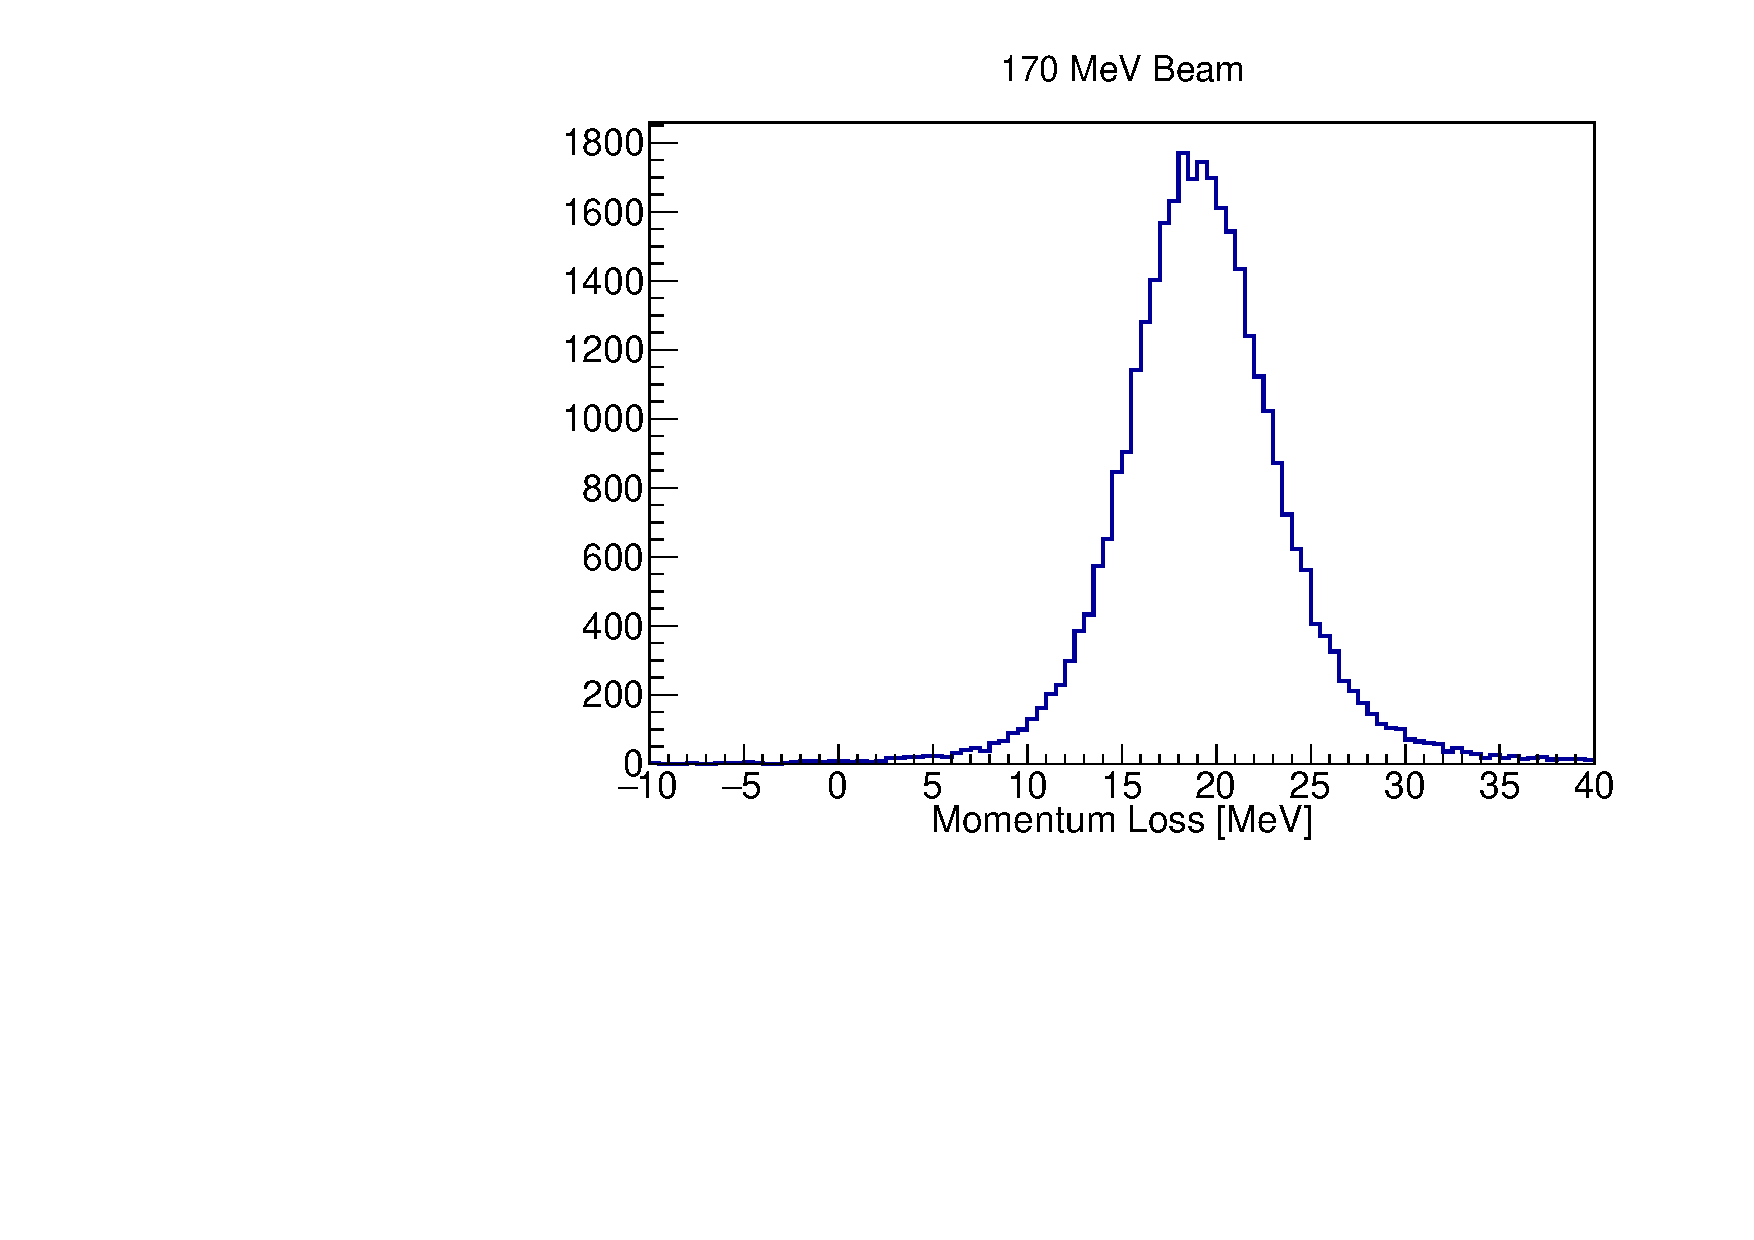
\includegraphics[width=0.45\textwidth]{11-Absorber/Figures/raw_170.pdf}\hfil
%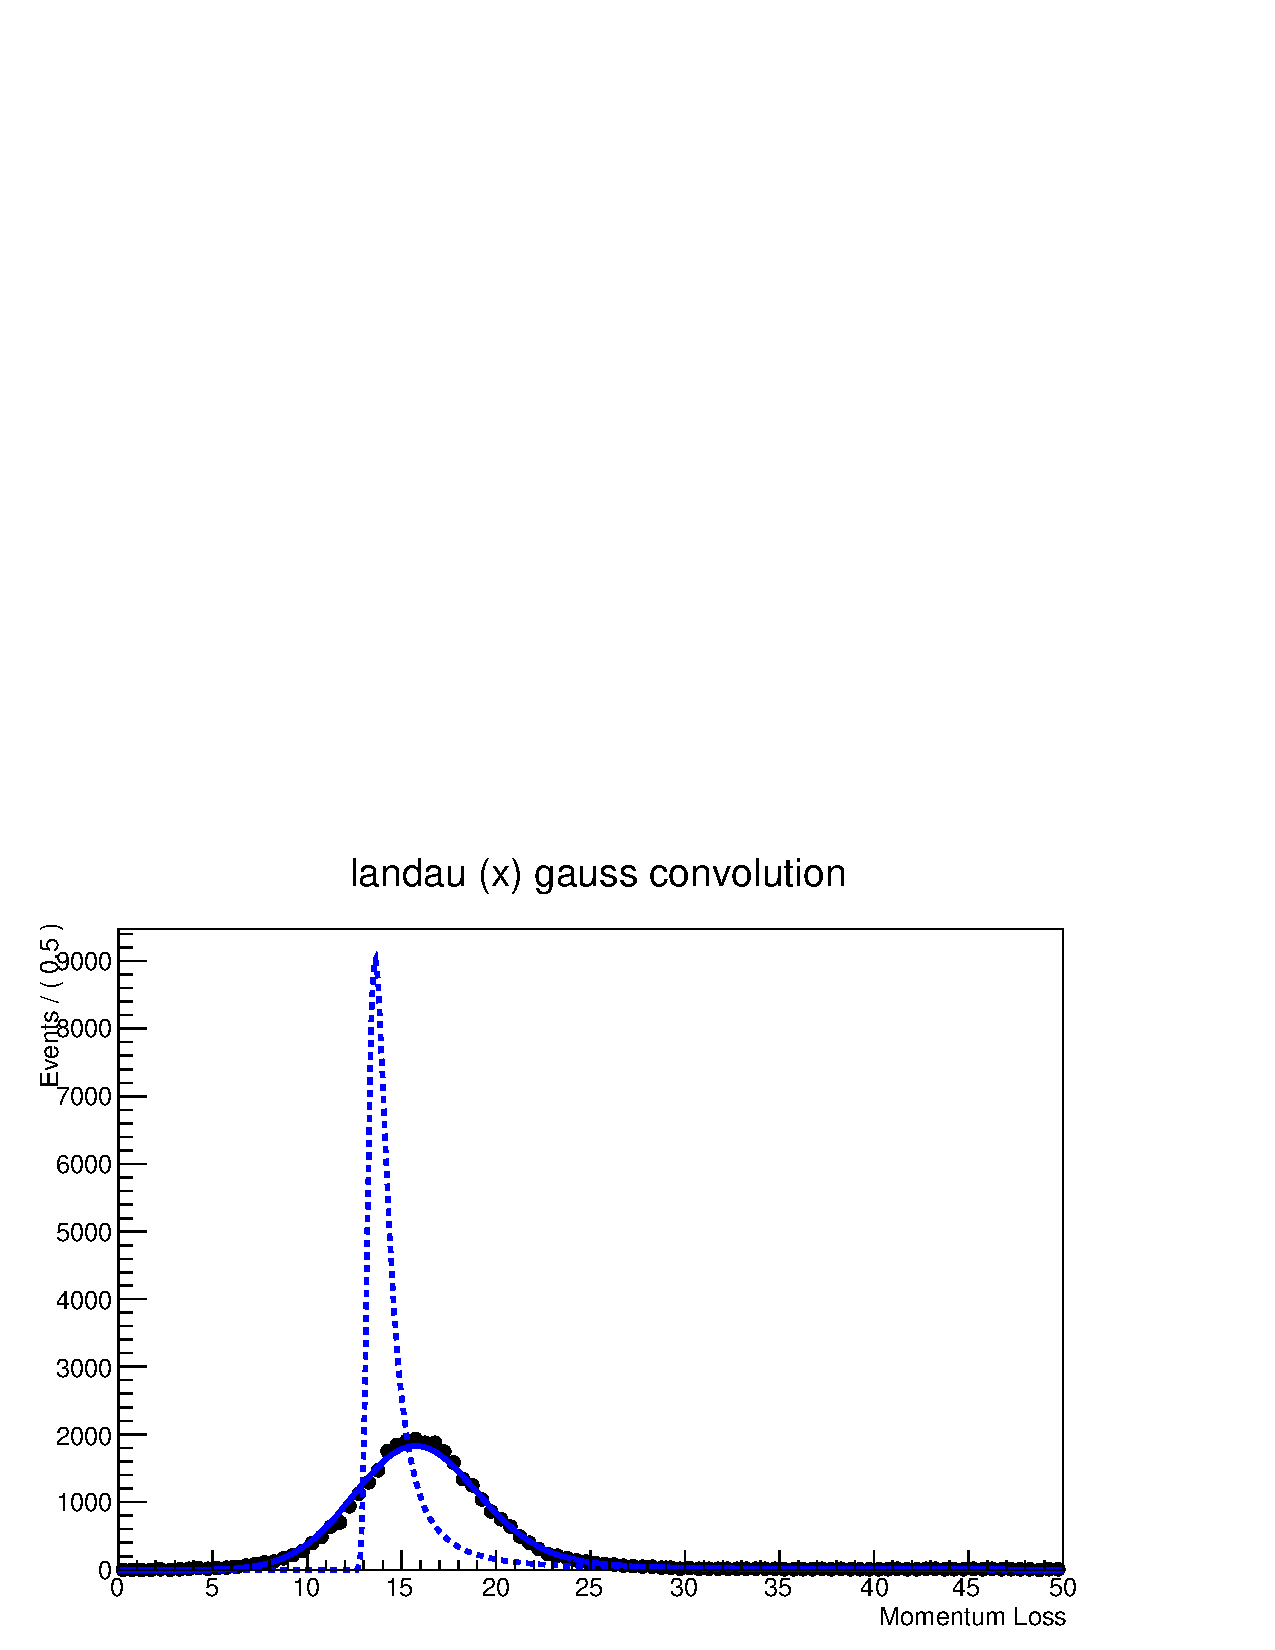
\includegraphics[width=0.45\textwidth]{11-Absorber/Figures/deconv_170.pdf}
%\vspace{-5cm}
%
%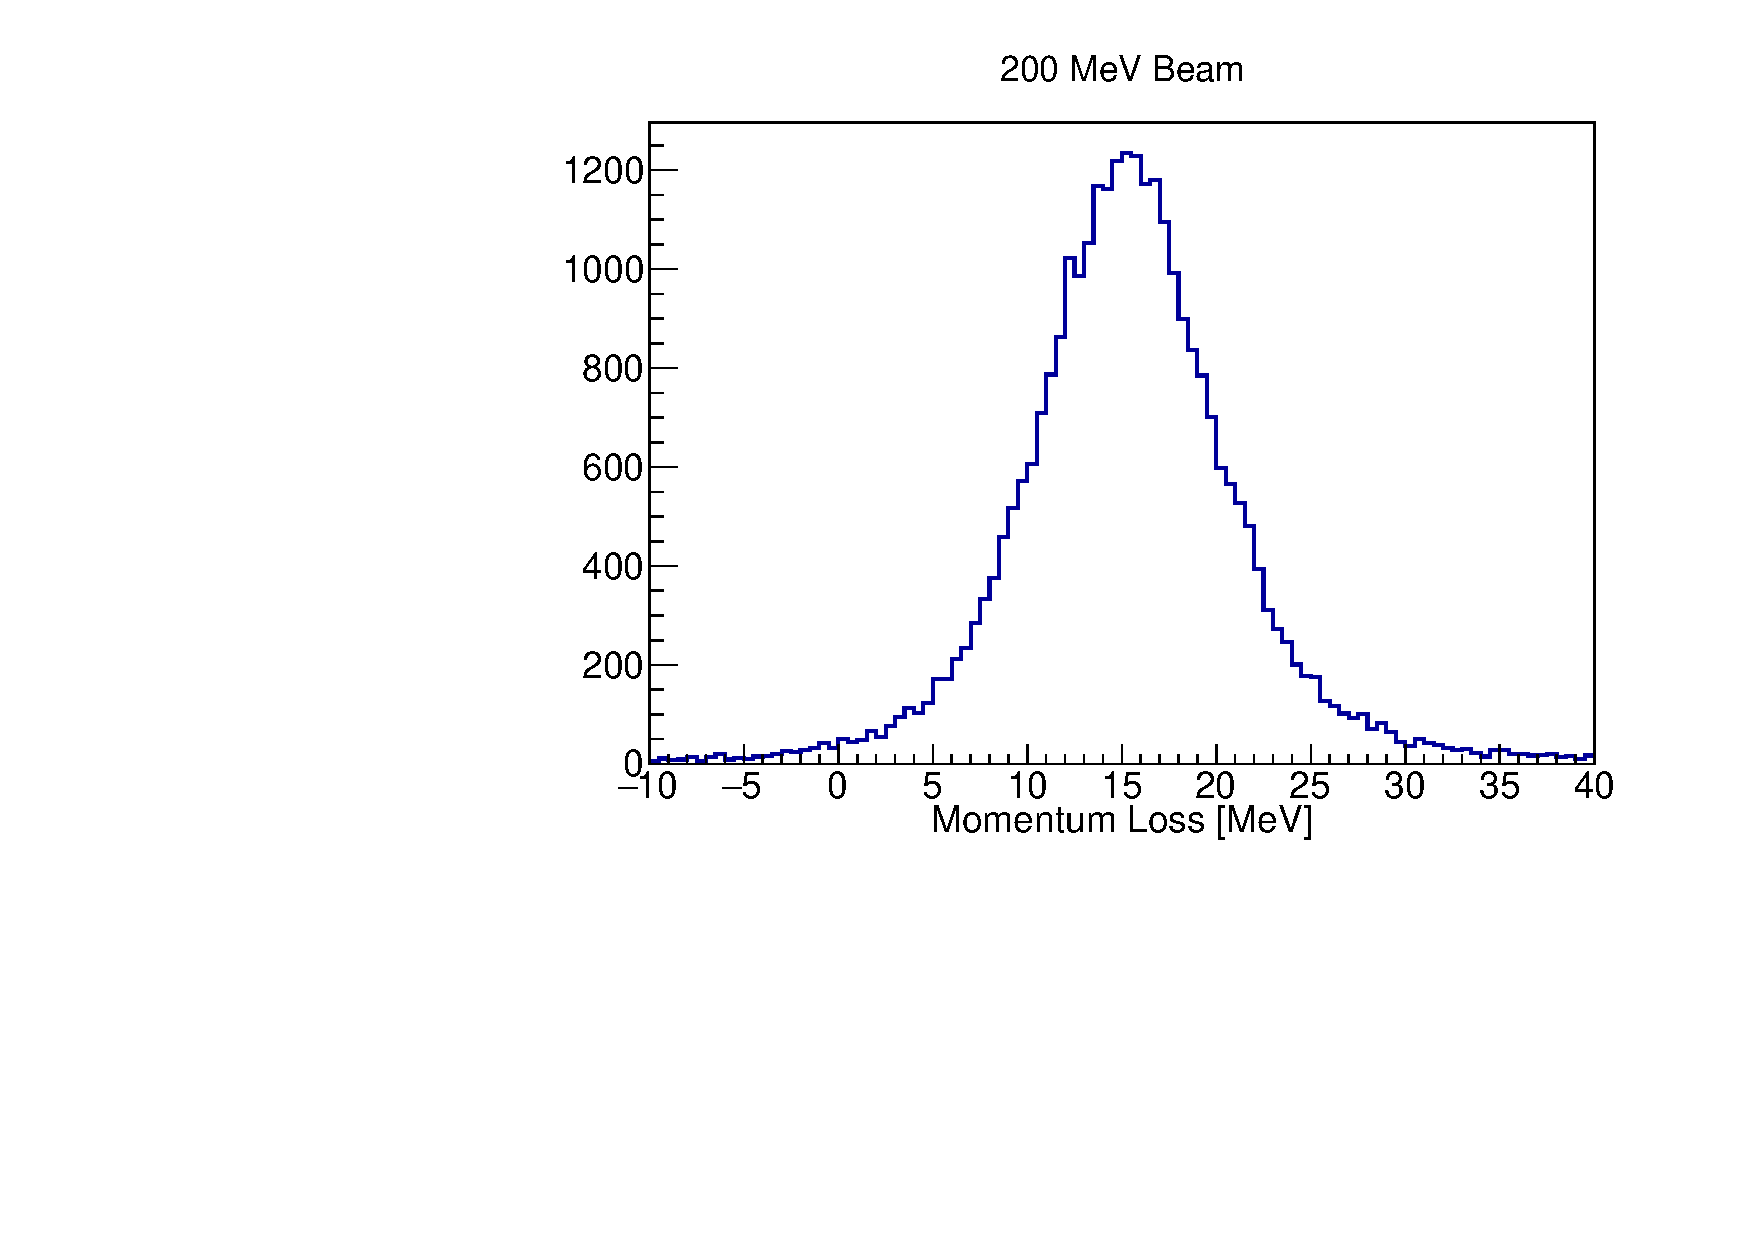
\includegraphics[width=0.45\textwidth]{11-Absorber/Figures/raw_200.pdf}\hfil
%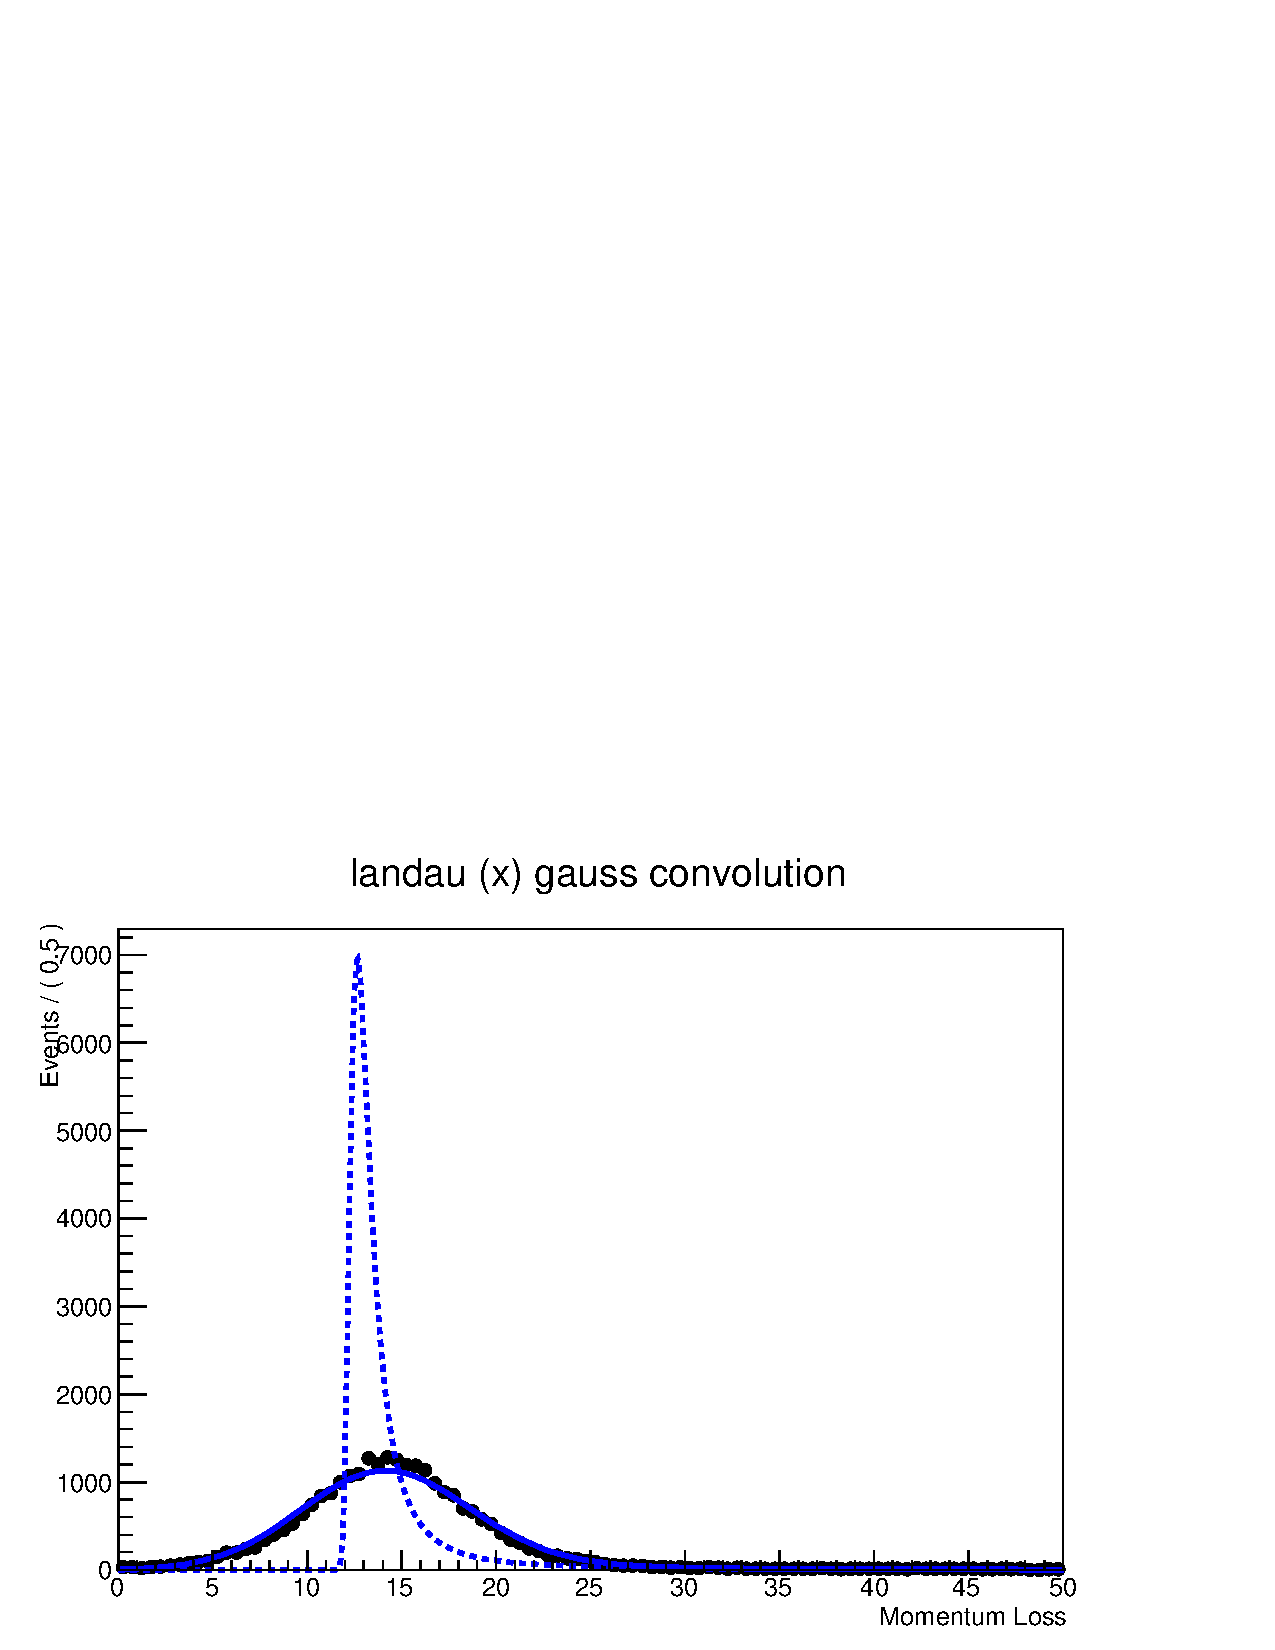
\includegraphics[width=0.45\textwidth]{11-Absorber/Figures/deconv_200.pdf}
%\vspace{-5cm}

%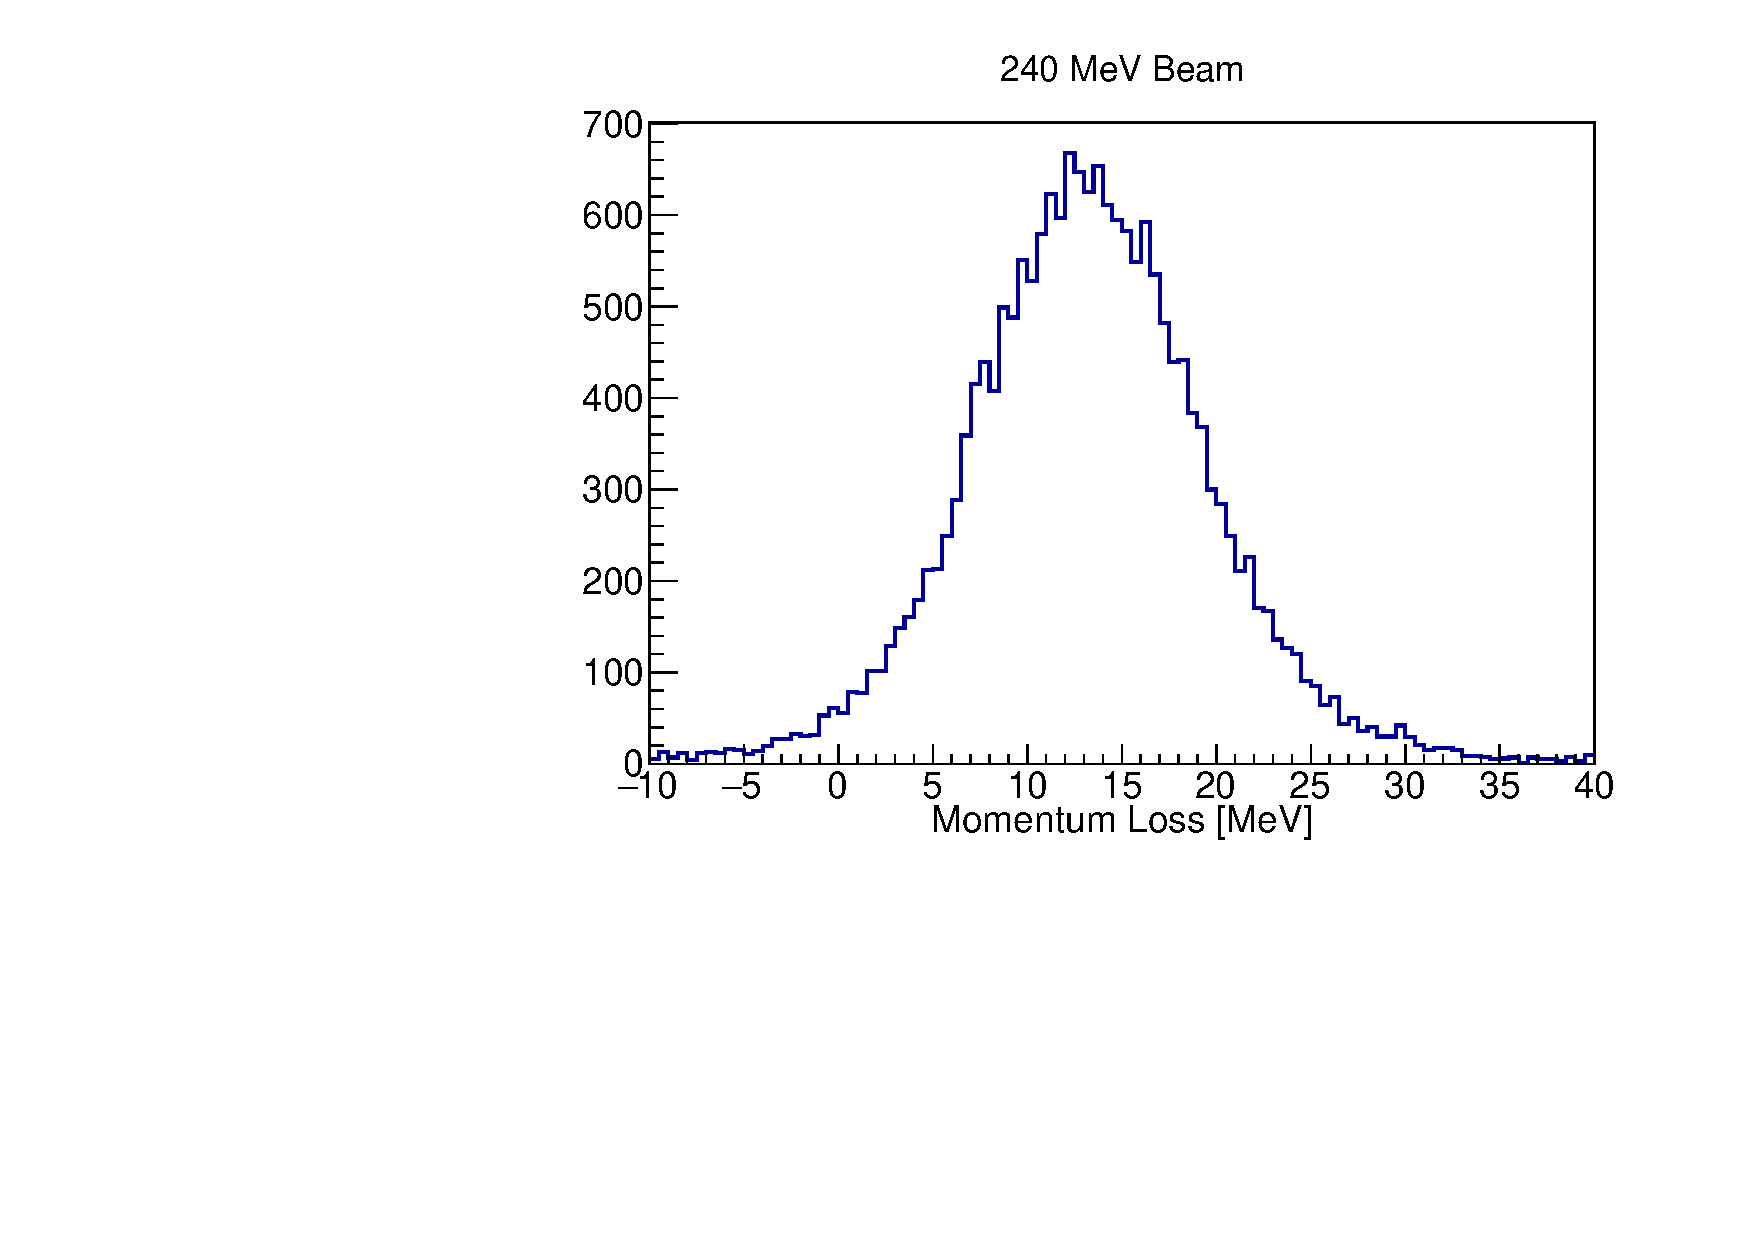
\includegraphics[width=0.45\textwidth]{11-Absorber/Figures/raw_240.pdf}\hfil
%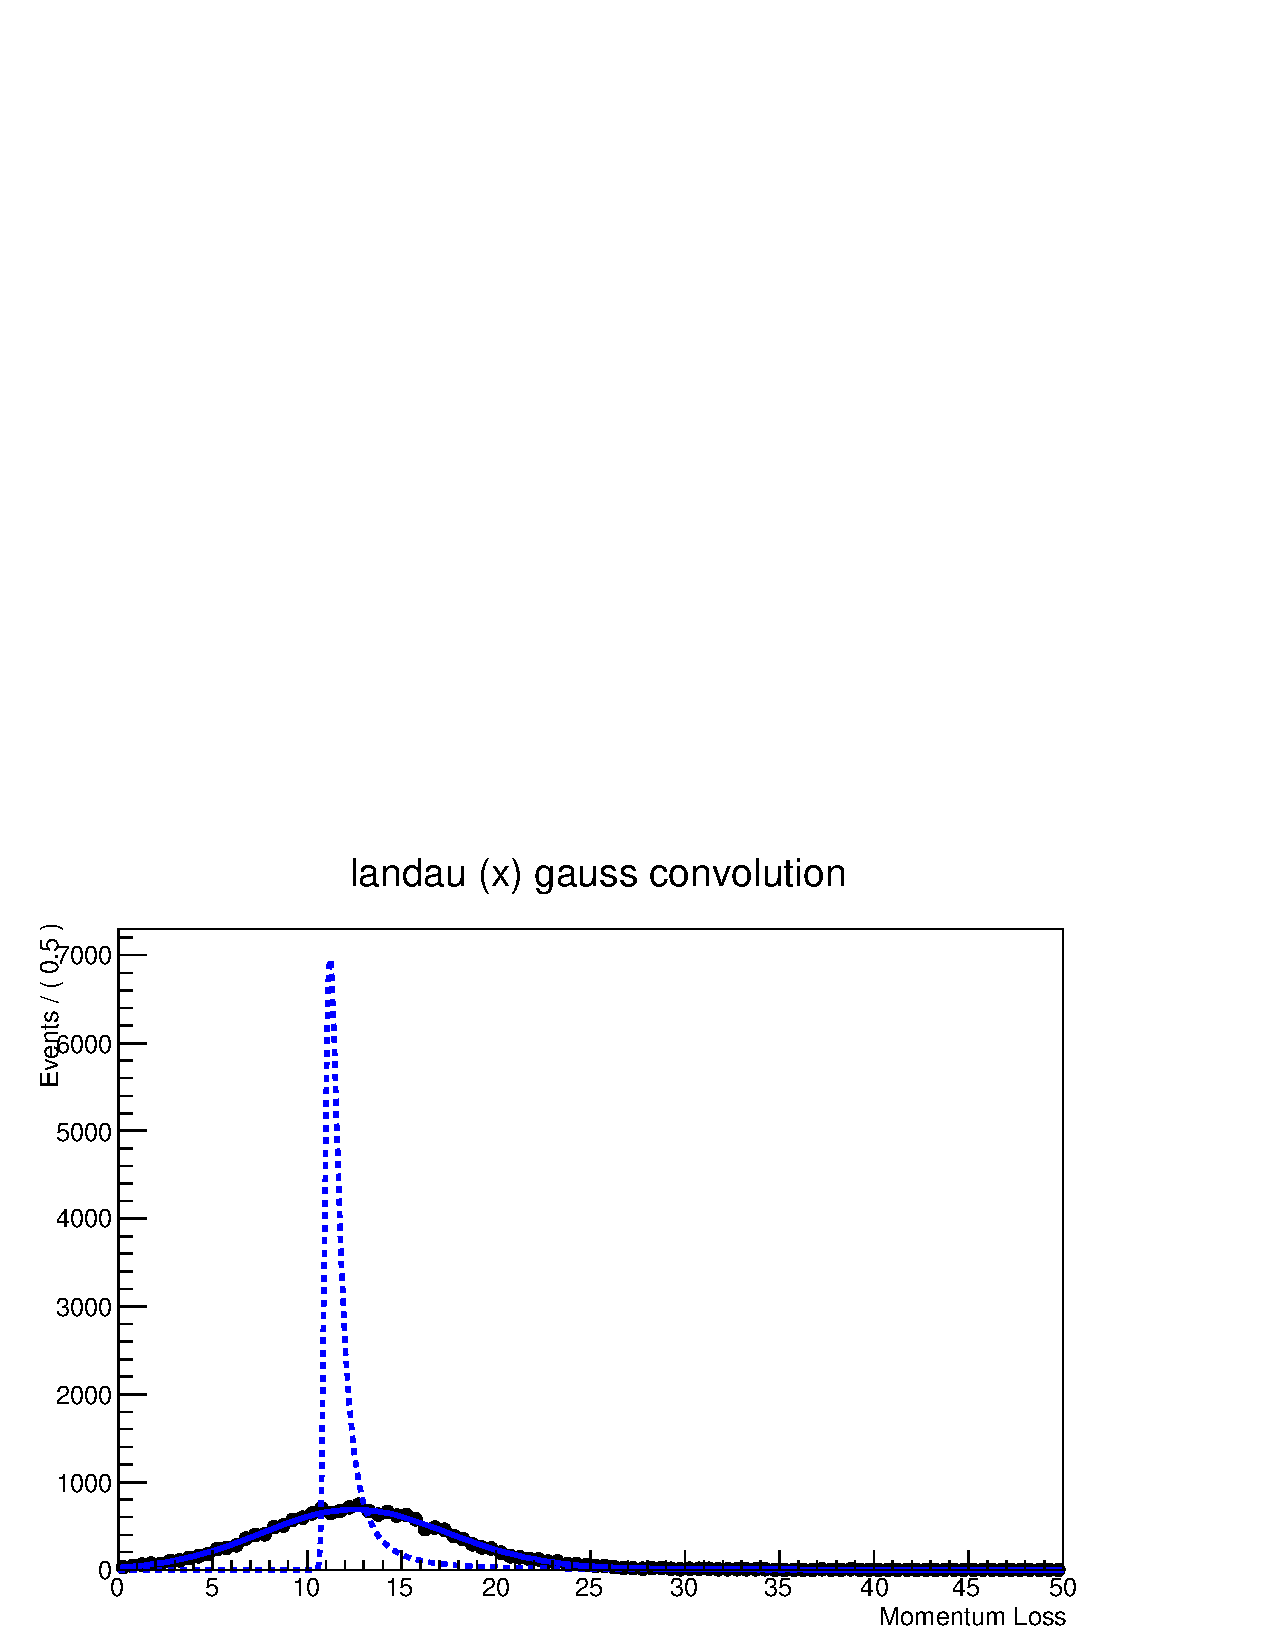
\includegraphics[width=0.45\textwidth]{11-Absorber/Figures/deconv_240.pdf}
%\caption{\label{fig:eloss_data} The measured momentum loss (left) and deconvolved distributions (right) in the MICE Lithium Hydride absorber.  Four different momentum settings are shown: 140 MeV(a), 170 MeV(b), 200 MeV(c), and 240 MeV(d).  The `deconvolved' plots show the data (black points), the fitted convolved landau and gaussian (solid blue line) and the landau by itself (dotted blue line).}
%\end{figure}

%The measurement of momentum loss is taken at four different beam momenta.  It agrees well with the Monte Carlo (in which the energy loss is modeled by GEANT) and with the predictions of the Bethe-Bloch formula, as shown in Figure~\ref{fig:eloss_bb}.

%{\color{red}
%\begin{itemize}
%\item add LH2 plots
%\item systematics
%\item more words about comparing with MC and Bethe-Bloch
%\end{itemize}
%}

%\begin{figure}
%\hfil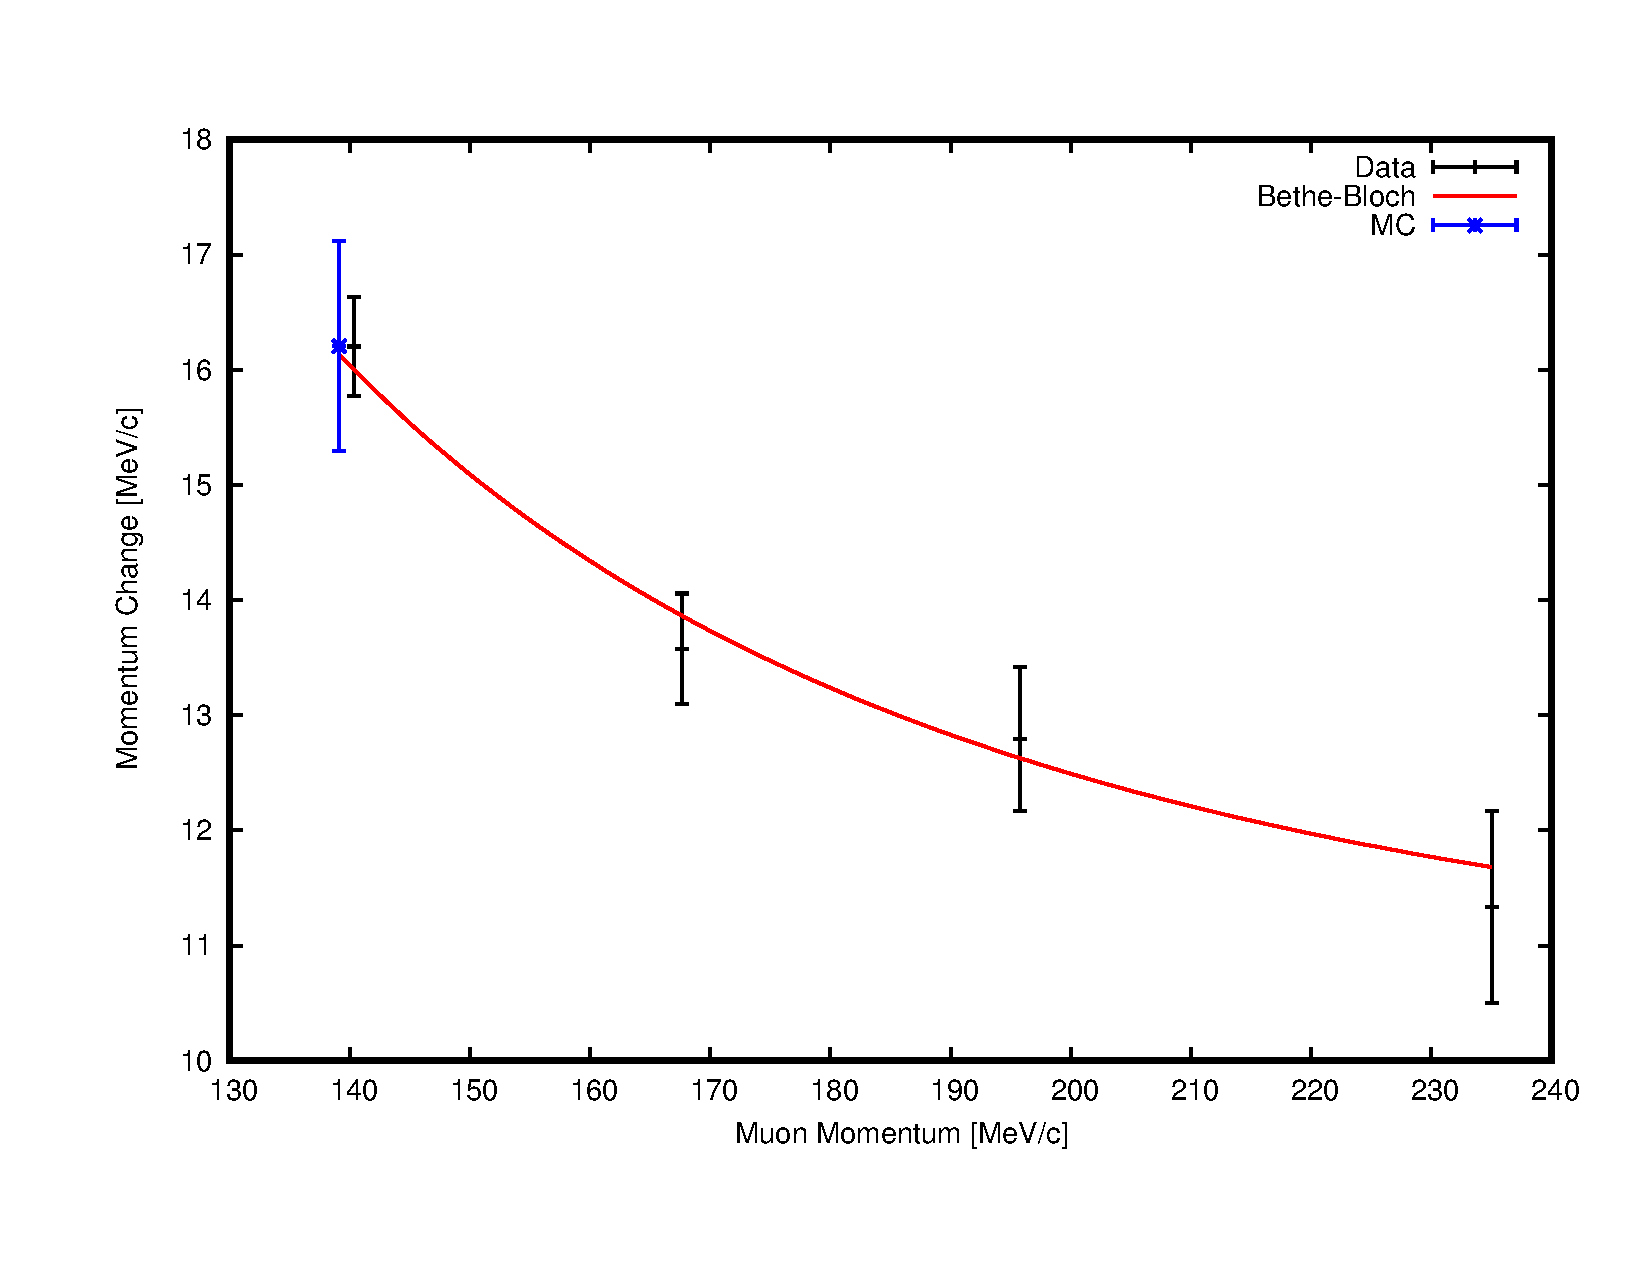
\includegraphics[width=0.45\textwidth]{11-Absorber/Figures/bb_compare.pdf}\hfil
%
%\caption{\label{fig:eloss_bb} Comparison of measured momentum loss in data and in MC in Lithium Hydride.  MPV of momentum loss is shown at each point with the% predition from the Bethe-Bloch formula shown as a solid line.}
%\end{figure}


%% Effect of error in geometry
%%   Test firing particles with modified geometry.
%%   Modified geometry in Scott's analysis.
 
